\subsection{Kafka}
	All'interno del progetto ThiReMa viene fatto uso della piattaforma Kafka per trasportare e trasformare i dati provenienti dai dispositivi verso le altre componenti del progetto.
	Per questo progetto è stato usato un singolo broker ma nulla vieta di estendere in un futuro Kafka creando un cluster con più broker.
	I principali topic che sono stati creati e che vengono utilizzati dalle vari componenti fino ad oggi sono:
	\begin{itemize}
		\item un topic per ogni gateway in cui vengono riversati i dati raccolti;
					%un topic per domarli
		\item un topic per gateway in cui vengono inviate le configurazioni dei gateway stessi;
					%un topic per trovarli
		\item un topic in cui vengono inseriti i messaggi di alert quando uno o più sensori superano delle 
		soglie stabilite.
					%un topic per ghermirli e nel buio incatenarli
	\end{itemize}
	Per effettuare il rilascio di questa componente è stato realizzato un file docker-compose (in cui sono presenti anche le altre componenti) che imposta automaticamente gli indirizzi e le porte in cui ascoltare e ricevere eventuali messaggi.
	Viene riportato sotto un piccolo estratto del file.

	\begin{figure}[H]
			\centering
			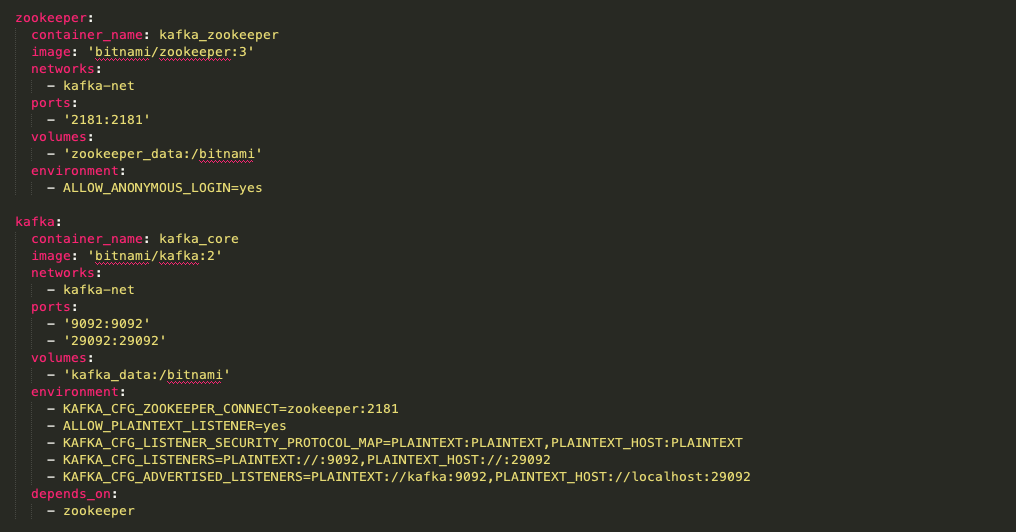
\includegraphics[scale=0.470]{res/images/estrattoKafka_dockerCompose.png}
			\caption{Estratto del file docker-compose.yml in cui viene impostato Kafka}
			\label{Immagine 1}
		\end{figure}		